\chapter{Pendahuluan}

\section{Gambaran Umum}
Pada praktikum ini, kita akan membangun sebuah purwarupa (prototype) sistem Machine Learning berbasis Computer Vision yang bertujuan untuk memprediksi secara dini kondisi kesehatan daun tomat. Praktikum ini menggunakan pendekatan end-to-end, mulai dari pemuatan data (\textit{data loading}) hingga fase \textit{deployment} dalam bentuk aplikasi web interaktif.

\begin{figure}[htbp]
    \centering
    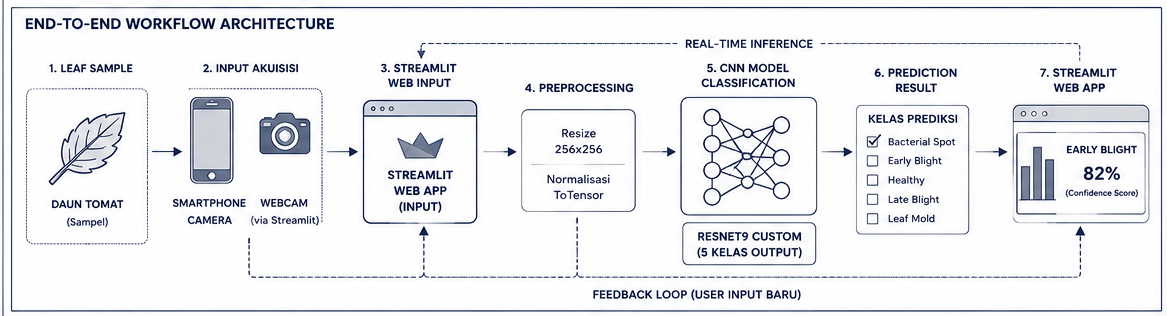
\includegraphics[width=0.9\textwidth]{gambar/end to end.png}
    \caption{Gambaran Alur Kerja (End-to-End Workflow)}
\end{figure}

Sebagaimana diilustrasikan pada Gambar 1.1, alur kerja dalam proyek Machine Learning ini merupakan proses berkesinambungan yang berawal dari pengumpulan dan penyiapan dataset daun tomat, diikuti proses perancangan serta pelatihan model jaringan saraf tiruan. Setelah model dievaluasi dan dianggap memadai, sistem diakhiri dengan proses integrasi (deployment) ke dalam platform aplikasi web interaktif agar model siap digunakan oleh para pengguna akhir.

Sistem ini dirancang tidak untuk memberikan diagnosis final layaknya pandangan pakar agrikultur, melainkan digunakan sebagai alat bantu \textit{screening} awal berdasarkan ciri-ciri visual yang tampak pada gambar daun.

\begin{figure}[htbp]
    \centering
    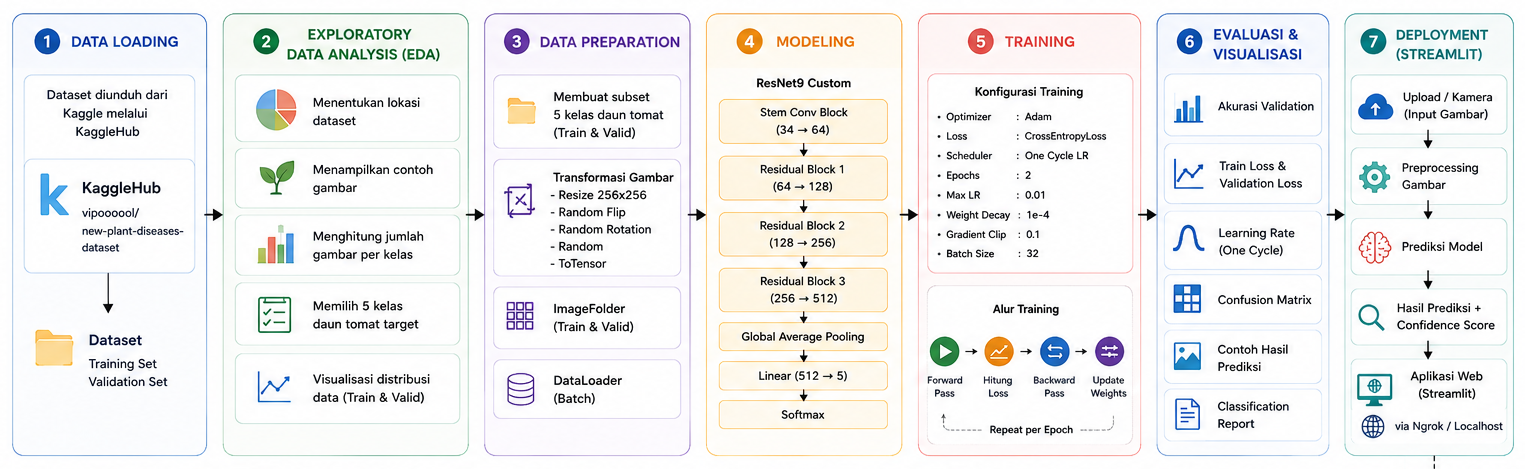
\includegraphics[width=0.85\textwidth]{gambar/pipe line.png}
    \caption{Detail Pipeline Pemrosesan Data dan Pemodelan}
\end{figure}

Lebih rinci lagi, struktur (pipeline) komputasi di bawah kap mesin dapat divisualisasikan pada Gambar 1.2. Alur komputasi ini memperlihatkan transformasi gambar asli ke dalam matriks angka (Tensor) yang sesuai dengan kerangka kerja PyTorch, yang selanjutnya akan diproses secara matematis oleh lapisan-lapisan (layers) pada model arsitektur ResNet9 guna membedakan pola penyakit pada daun tomat.

\section{Tujuan Praktikum}
Adapun tujuan utama dari pelaksanaan praktikum ini adalah sebagai berikut:
\begin{enumerate}
    \item Memberikan pengalaman praktik alur kerja (workflow) pembuatan model Machine Learning secara utuh.
    \item Membuat model Machine Learning untuk mengklasifikasikan gambar daun tomat.
    \item Menampilkan hasil prediksi model dalam bentuk aplikasi web sederhana.
    \item Memahami bahwa model memiliki batasan dan hanya valid untuk data yang sesuai dengan domain pelatihan.
\end{enumerate}

\section{Batasan Sistem}
Untuk memastikan fokus pembelajaran tetap terarah, sistem yang akan dibangun memiliki beberapa batasan:
\begin{itemize}
    \item Dataset difokuskan secara eksklusif pada \textbf{5 kelas kondisi daun tomat}:
    \begin{enumerate}
        \item Bacterial Spot
        \item Early Blight
        \item Late Blight
        \item Leaf Mold
        \item Healthy (Sehat)
    \end{enumerate}
    \item Sistem tidak dapat digunakan untuk memprediksi jenis tanaman lain.
    \item Model yang dilatih belum dilengkapi dengan kelas penolakan (seperti kelas `Unknown` atau `Non Leaf`), sehingga input gambar diasumsikan selalu berupa daun tomat.
\end{itemize}

\section{Persiapan Lingkungan Praktikum}
Pada praktikum ini, spesifikasi komputer lokal yang tinggi tidak diwajibkan karena seluruh proses komputasi, termasuk pelatihan model yang membutuhkan GPU, akan dilakukan di \textit{cloud}. Berikut adalah \textit{tools} dan lingkungan yang perlu dipersiapkan:

Berikut adalah rincian masing-masing teknologi yang menjadi tulang punggung praktikum ini:

\begin{itemize}
    \item \textbf{Google Colab}: Lingkungan Jupyter Notebook gratis berbasis cloud dari Google yang menyediakan akses ke GPU. Digunakan untuk mengeksekusi kode Python, melatih model, dan menjalankan *server* aplikasi.
    \item \textbf{KaggleHub}: Library untuk mengunduh dataset secara langsung dari Kaggle ke environment Google Colab.
    \item \textbf{PyTorch dan Torchvision}: Framework Deep Learning yang akan digunakan untuk mengelola dataset dan membangun arsitektur jaringan saraf tiruan (ResNet9).
    \item \textbf{Streamlit}: Framework open-source berbasis Python untuk membuat antarmuka web interaktif khusus Machine Learning.
    \item \textbf{Ngrok}: Layanan \textit{tunneling} yang memungkinkan aplikasi Streamlit yang berjalan di \textit{localhost} Google Colab dapat diakses melalui internet menggunakan tautan publik.
\end{itemize}

Pastikan Anda telah memiliki akun Google untuk menggunakan Google Colab. Pada bab selanjutnya, kita akan mulai mempersiapkan *environment* praktikum.
